\documentclass[12pt,a4paper]{article}
\usepackage[UTF8]{ctex}
\usepackage{geometry}
\usepackage{graphicx}
\usepackage{amsmath,amssymb}
\usepackage{fancyhdr}
\usepackage{titlesec}
\usepackage{setspace}
\usepackage{indentfirst}
\usepackage{cite}
\usepackage{caption}
\usepackage{hyperref}
\usepackage{enumitem}
\usepackage{multirow}
\usepackage{longtable}
\usepackage{booktabs}
\usepackage{makecell}
\usepackage{multicol}
\usepackage{float}
\usepackage{subfigure}
\usepackage{adjustbox}

% 页面设置
\geometry{a4paper, left=2.5cm, right=2.5cm, top=2.5cm, bottom=2.5cm}
\setlength{\parindent}{2em}
\linespread{1.25}
\pagestyle{fancy}
\fancyhf{} % 清除页眉页脚
\cfoot{\thepage} % 页码居中
\renewcommand{\headrulewidth}{0pt} % 去掉页眉横线

% 标题格式设置
\titleformat{\section}{\centering\zihao{4}\heiti}{\thesection}{1em}{}
\titleformat{\subsection}{\zihao{-4}\heiti}{\thesubsection}{1em}{}
\titleformat{\subsubsection}{\zihao{-4}\heiti}{\thesubsubsection}{1em}{}

% 正文小四宋体
\renewcommand{\normalsize}{\zihao{-4}\songti\linespread{1.25}\selectfont}

% 摘要页为第一页
\begin{document}

% 第一页 摘要页
\thispagestyle{empty}
\begin{center}
    \zihao{3}\heiti基于Delaunnay三角剖分的康养资源分布情况分析 \\
    \vspace{1em}
    \zihao{4}\heiti选题编号:A \\
    \quad 队伍编号:202503192 \\
\end{center}

\vspace{2em}

\noindent\textbf{摘要:}本文围绕康养城市建设问题,针对康养资源分布不均、医养融合深度不够等问题,建立了康养指标模型,并结合上海市16市、常州、南京、海口、广州的医院、养老院分布结合2024中国康养城市100强名单等进行了实证研究。首先,通过计算简化版的康养指标得出康养指标得分越高的城市该城市在名单中的排名越高,推出建立的简化模型可以在一定程度上工作;接着,利用python批量带入数据进一步验证了模型的有效性;最后对常州、广州、南京、海口、上海五个城市进行了Delaunay三角剖分进行空间分布分析。研究结果表明该模型能很直观地反映康养资源的分布情况,对于资源分布调整及建设有很大帮助。本研究对城市规划,GIS相关,资源配置等具有一定的参考价值。

\vspace{1em}

\noindent\textbf{关键词:}Delaunay三角剖分;康养城市;资源配置;空间分布;熵值法

\newpage

% 正文
\section{引言}

随着我国人口老龄化进程加快,康养城市建设正逐步成为推动社会
可持续发展的重要战略方向。在2025年全国两会期间,
多位代表委员聚焦康养议题,提出诸如盘活空置房、
发展数字家庭、推动医养融合等富有前瞻性的建议,
引发社会广泛关注。各地政府亦积极响应,
安徽出台《关于支持康养产业高质量发展的意见》\cite{01},
广德市加快“康养名城”建设步伐,吉林提出打造旅居康养目的地,
种种举措展现出康养城市建设已从政策倡导迈向系统实践。
然而,现实中康养城市建设仍面临诸多挑战:
康养资源在区域间分布不均,智慧养老技术应用滞后,
医养融合程度不足,制约了康养服务体系的整体效能。
因此,科学评估当前康养资源配置状况,构建合理的评价体系,
并设计优化资源配置的策略,成为推进康养城市高质量发展的当务之急。
为此,本文将围绕以下三方面开展研究:

\textbf{一、对城市康养资源分布现状进行分析,揭示资源配置的短板与优化空间;}

\textbf{二、构建康养城市综合评价模型,量化城市康养发展水平;}

\textbf{三、建立康养资源优化配置模型,制定切实可行的实施策略,旨在为地方政府推动康养城市建设提供科学依据与决策支持。}

\begin{multicols}{2}

\section{模型建立}

\subsection{康养指标选取标准}

(1) 相关性:指标应与康养城市建设密切相关,能够反映康养资源的配置状况。

(2) 可获取性:指标数据应易于获取,确保模型的可操作性。

(3) 代表性:指标应具有一定的代表性,能够反映城市整体的康养发展水平。

(4) 可比性:指标应具有一定的可比性,便于不同城市之间进行横向比较。

(5) 时效性:指标数据应具有一定的时效性,能够反映当前的康养资源配置状况。

(6) 可量化性:指标应具有一定的可量化性,便于进行定量分析。

(7) 适用性:指标应适用于不同类型的城市,具有一定的普遍适用性。

\subsection{康养指标}

(1) 生活环境:良好的生活环境有助于减少疾病传播、改善心理状态、提高生活质量,是维持身体健康的重要基础。

(2) 医疗服务:医疗服务能及时预防、诊断和治疗疾病,提升健康管理水平,有效降低死亡率和患病风险,是保障公众健康的关键力量。

(3) 经济水平:经济水平决定了医疗保障、营养摄入和生活质量,高水平经济可提供更完善的健康服务体系,为居民健康提供有力支撑。

(4) 人口结构:人口结构影响健康资源需求与配置,老龄化社会需更多医疗与养老服务,合理的人口结构有助于实现健康服务的可持续发展。

(5) 生活成本:生活成本影响人们获取健康食物、医疗服务与良好居住条件的能力,成本过高可能导致压力增加和健康资源不足,从而危害身心健康。

(6) 教育资源:教育资源提升健康意识与自我管理能力,促使人们养成良好生活习惯,有助于预防疾病、改善心理健康,从根本上促进全民健康水平。

(7) 社区服务:社区服务能提供便捷的医疗、养老、心理支持等服务,增强居民健康管理与应急能力,是提升全民健康水平的重要基础设施。

\subsection{量化康养指标}

\subsubsection{资源密度}
\[
\rho = \frac{R}{S}
\]

其中,$\rho$为资源密度,$R$为资源总量,$S$为区域面积。

\subsubsection{人口密度}
\[
\delta = \frac{P}{S}
\]

其中,$\delta$为人口密度,$P$为区域人口总数,$S$为区域面积。

\subsubsection{资源配置密度/人均资源数量}
\[
E = \frac{\rho}{\delta}\cdot 10^5=\frac{R}{P}\cdot 10^5
\]

其中,$E$为资源配置均衡度,$10^5$校准数量级,$R$为资源总量,$P$为区域人口总数。\textbf{当$E$越大,说明人均资源越丰富。}

\subsubsection{康养资源倾斜度}

\[
W=\frac{R}{C}
\]

其中,$W$为康养资源倾斜度,$R$为资源总量,$C$为年人均收入。

\subsubsection{资源分配系数}

\[
G=\frac{R}{P\cdot C}
\]
其中,$G$为资源分配系数,$R$为资源总量,$P$为区域人口总数,$C$为年人均收入。

\subsubsection{资源配置合理性}
\[
\sigma = \sqrt{\frac{1}{n} \sum_{i=1}^{n}(G_i - \overline{G})^2}
\]
其中,$\overline{G} = \frac{1}{n} \sum_{i=1}^{n}G_i$,是全体$G$的均值,$E_i$为第i个城市的资源配置密度,n为数据数量(个数),$\sigma$为全体E的方差,代表资源配置合理性。\textbf{当$\sigma$越小,说明资源配置越合理。}

\subsubsection{考虑地理因素下的资源配置合理性}

在考虑地理因素的情况下,我们需要引入地理位置对资源配置的影响。地理位置已经由百度地图开放平台获取。将经纬度转化为平面坐标系下的坐标点,使用\textbf{Delaunay三角剖分}方法对上海市的医院进行空间分析。

Delaunay三角剖分能够有效地将空间中的点集划分为一系列三角形,使得每个三角形的顶点都是点集中的点,并且满足某些几何性质,如最大化最小角度等。这种方法在地理信息系统(GIS)中被广泛应用,可以用于分析空间数据的分布特征、计算邻近关系等。

\begin{figure}[H] %H为当前位置,!htb为忽略美学标准,htbp为浮动图形
\centering %图片居中
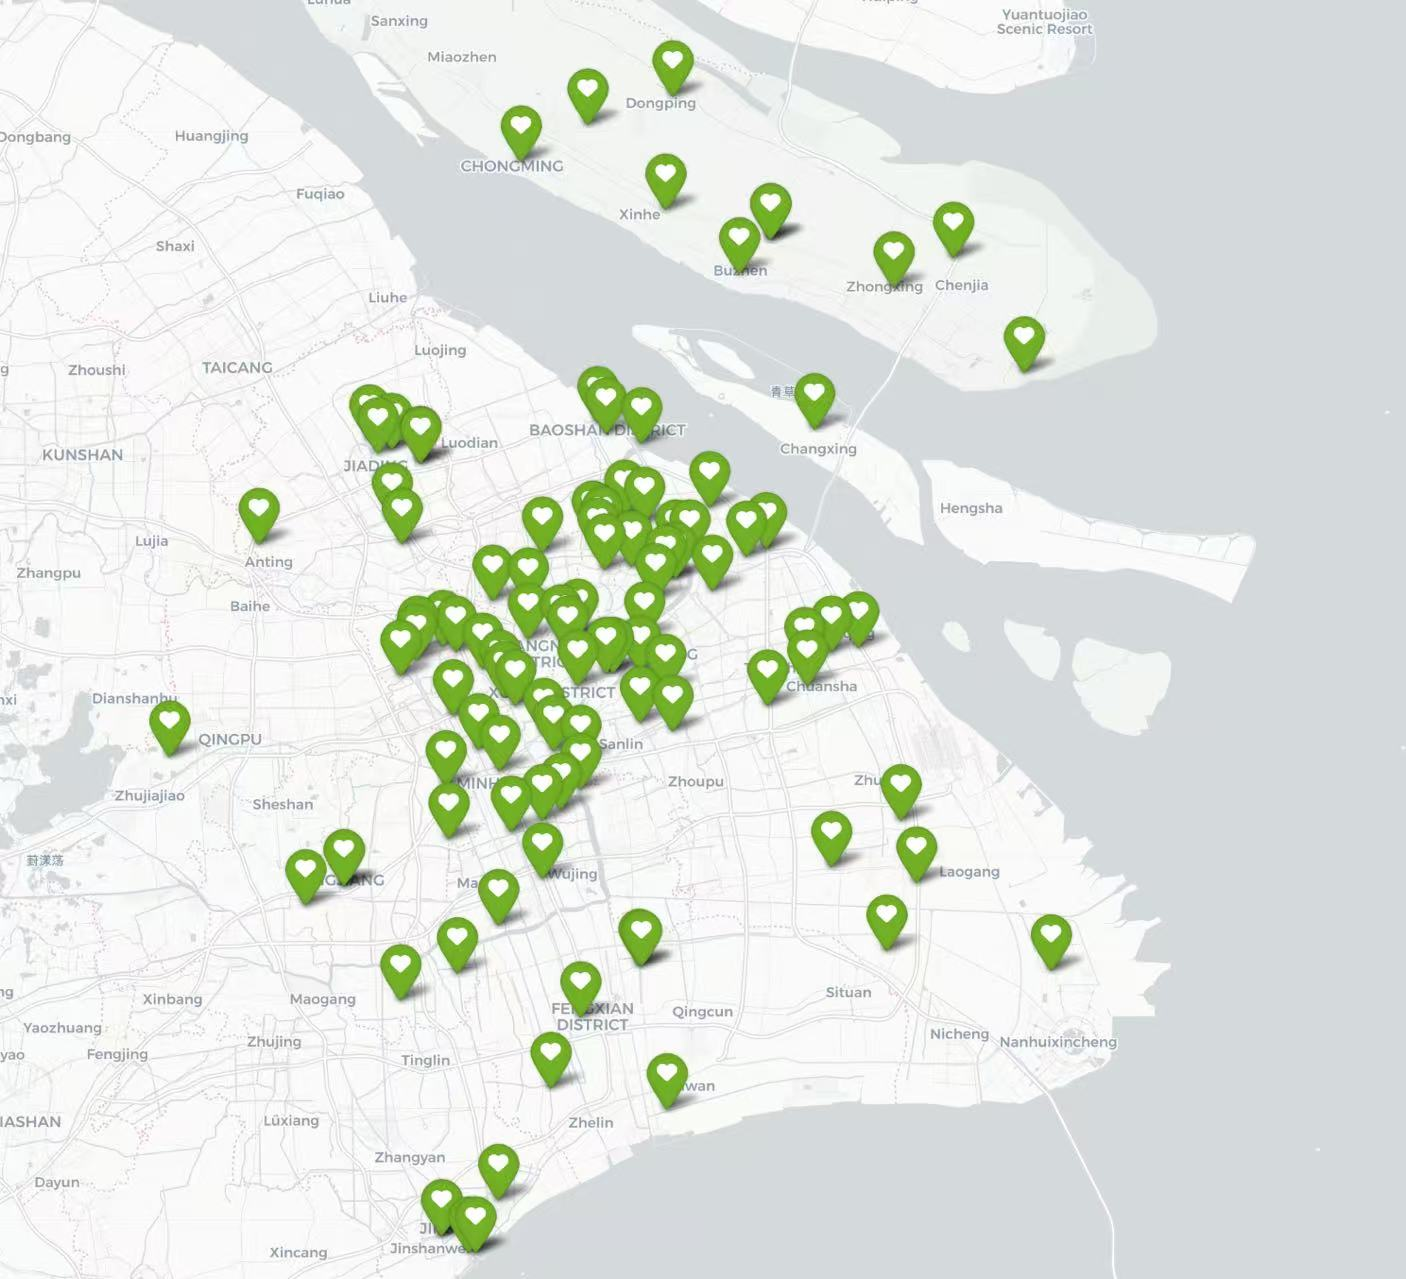
\includegraphics[width=0.5\textwidth]{images/shanghai_hospital_location.jpg} %插入图片,[]中设置图片大小,{}中是图片文件名
\caption{上海医院坐标的散点图} %最终文档中希望显示的图片标题
\label{Fig.main2} %用于文内引用的标签
\end{figure}

为了得到资源分布合理性$G$的信息,我们选取以下几个指标:

(1) 剖分三角面积$S$:当剖分三角面积$S$越大,说明资源分布越稀疏;当$S$越小,说明资源分布越密集。

\it程序在这一步会获得当前三角形的面积,三角形重心的坐标点,对坐标进行逆地理编码,获得坐标所在区级行政区域,以此该区域的人口密度以及人均收入。
\normalfont

(2) 人口数量$P$:当人口数量$P$越大,说明该区域的人口越密集,资源需求越大。

(3) 人均收入$C$:当人均收入$C$越高,说明该区域的经济水平越高,居民获取资源的能力越强。

\begin{figure}[H] %H为当前位置,!htb为忽略美学标准,htbp为浮动图形
\centering %图片居中
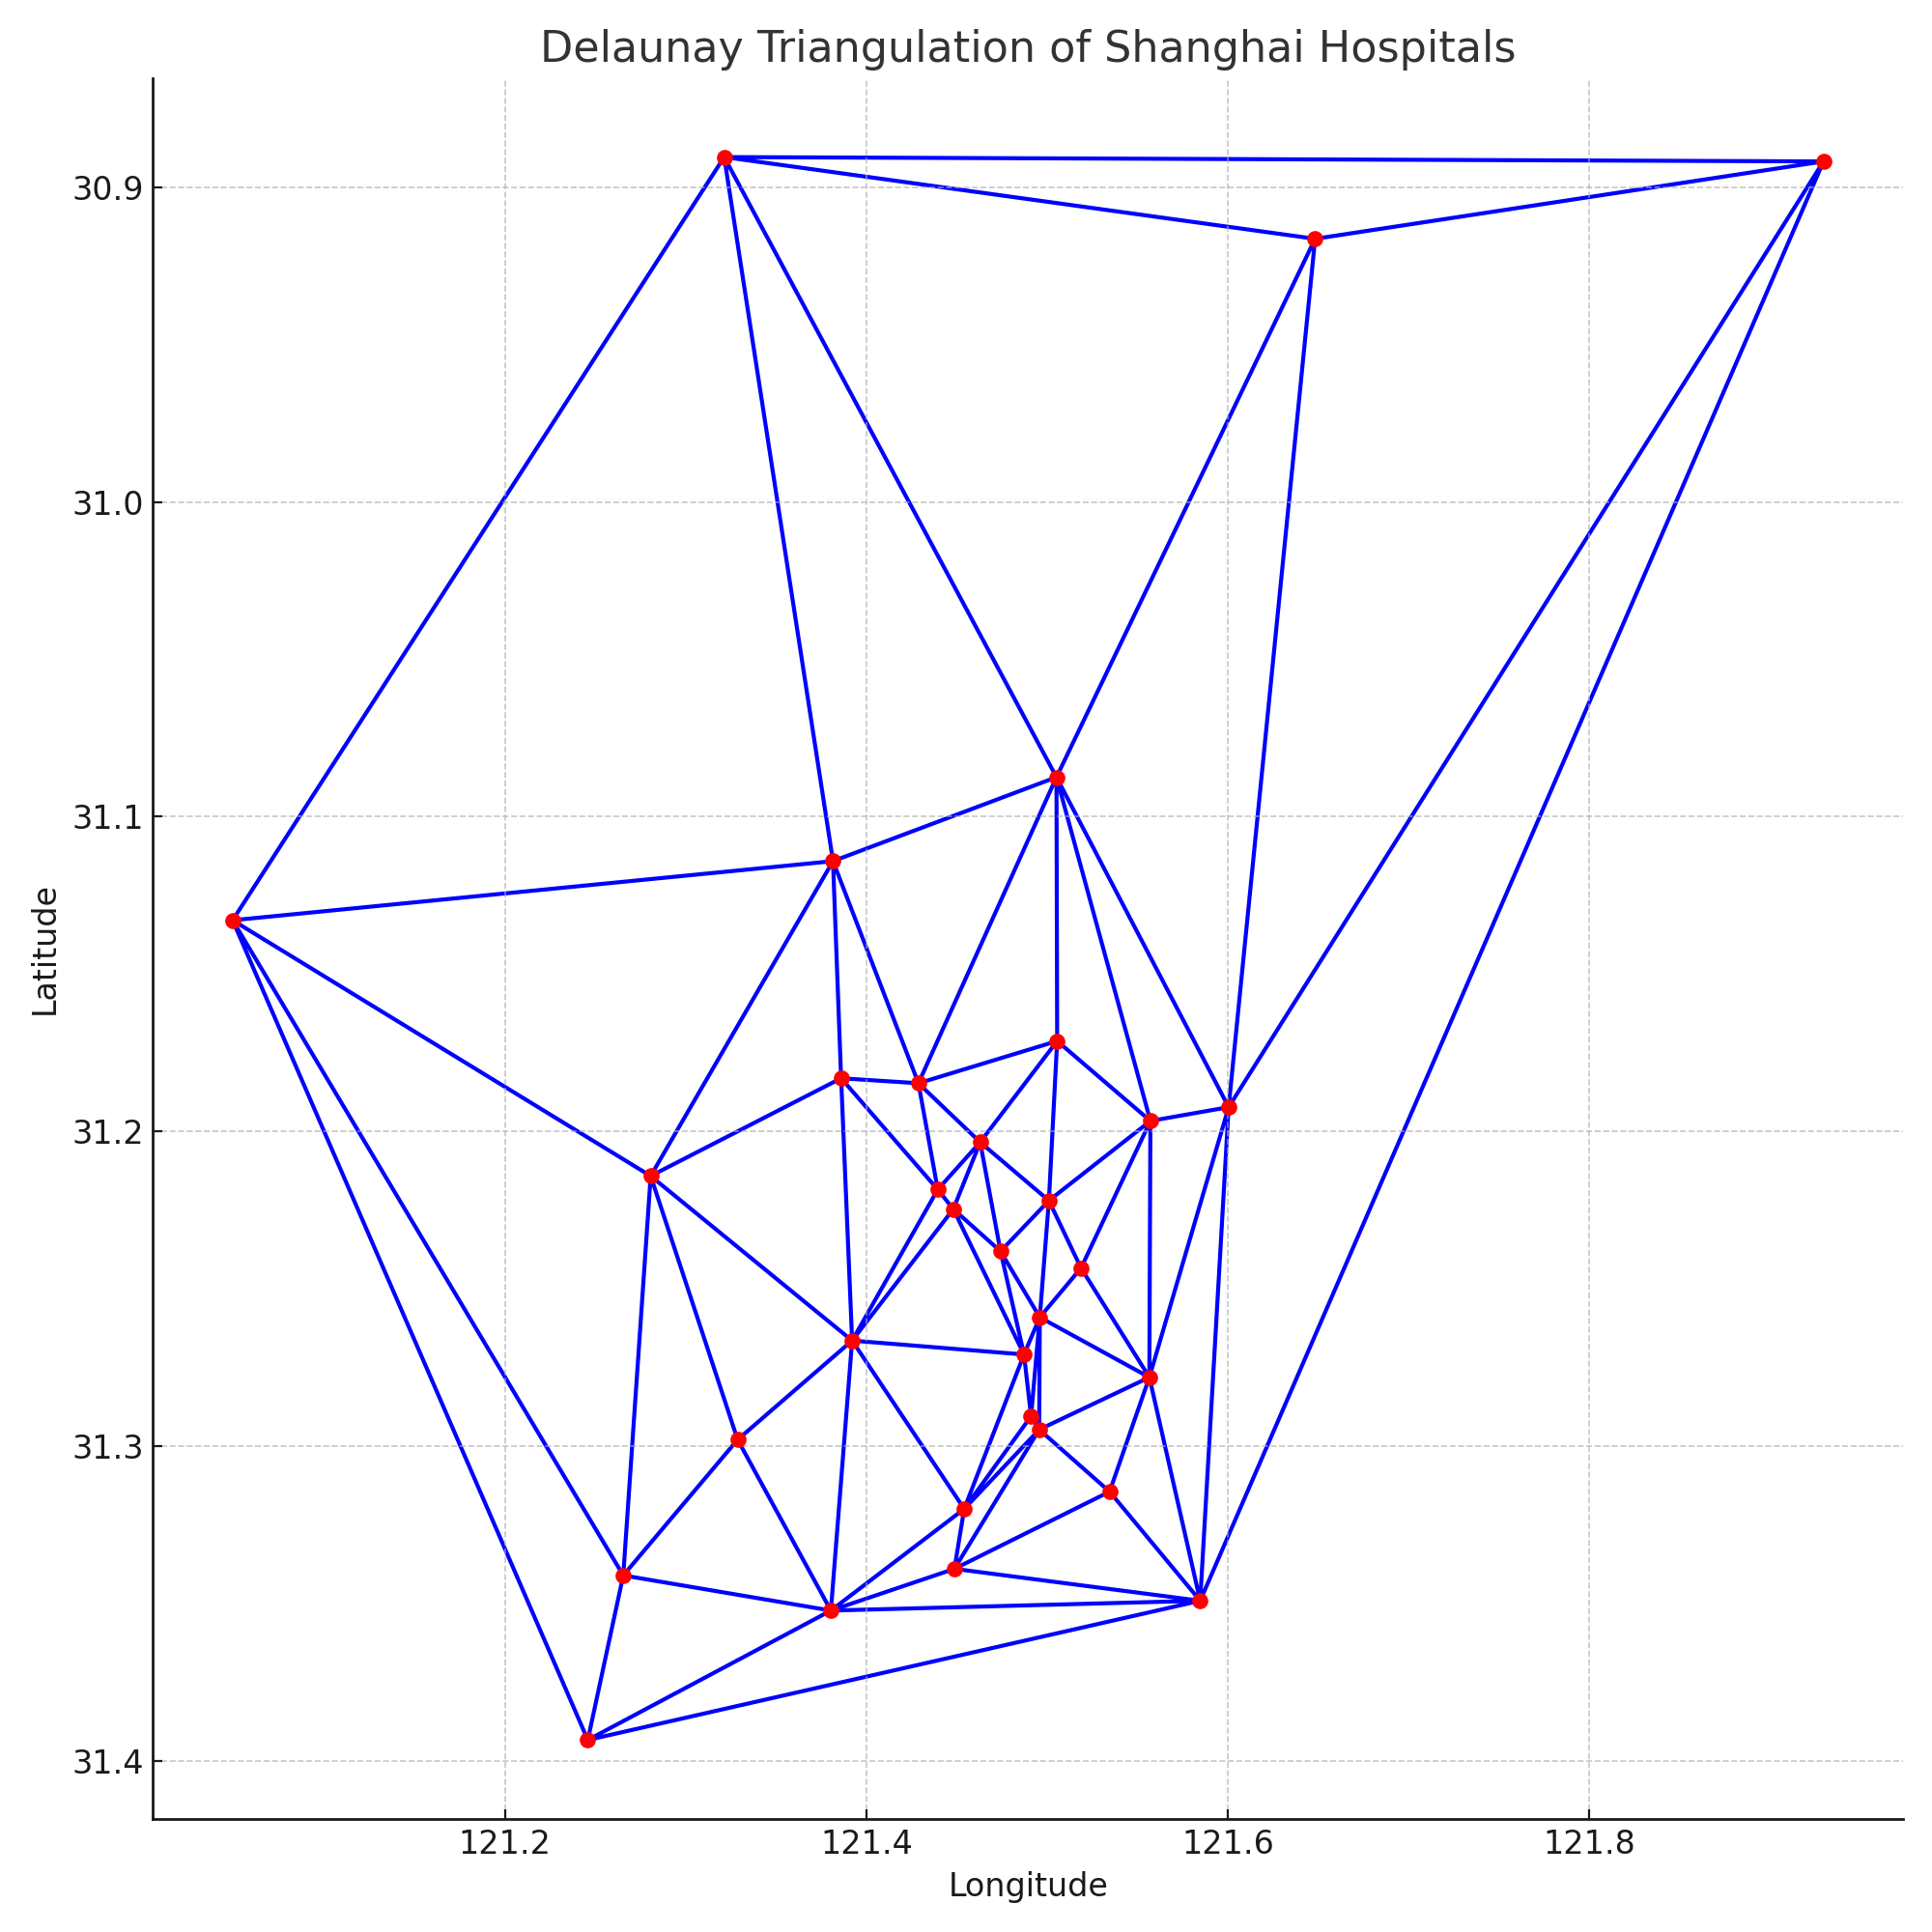
\includegraphics[width=0.5\textwidth]{images/delaunay_triangulation_shanghai.png} %插入图片,[]中设置图片大小,{}中是图片文件名
\caption{部分上海医院坐标的三角剖分示意图} %最终文档中希望显示的图片标题
\label{Fig.main2} %用于文内引用的标签
\end{figure}

于是我们可以定义一个新的资源配置合理性指标$B$,综合考虑以上三个因素:
\[
B = \frac{k}{S\cdot P \cdot C}
\]

其中,$B$为资源配置合理性指标,$S$为剖分三角面积,$P$为人口数量,$C$为人均收入,$k$为常数。

由于$P=\rho \cdot S$,$\rho$为人口密度,因此可以将$B$重写为

\[
B = \frac{k}{S^2 \cdot C \cdot \rho}
\]

理想情况下,$B$应趋于一个常数。\textbf{$B$过高或过低都说明资源配置不合理。}

\subsubsection{资源配置均衡度}

为了衡量所有$B$趋近某个常数的程度,我们可以定义资源配置均衡度$I$为:

\[
I = \sqrt{\frac{1}{n} \sum_{i=1}^{n}(B_i - \overline{B})^2}
\]

其中,$\overline{B} = \frac{1}{n} \sum_{i=1}^{n}B_i$为全体$B$的均值,$I$为资源配置均衡度,$n$为数据数量(个数),$B_i$为第$i$个城市的资源配置均衡度指标。

\subsection{简化的康养指数}

在实际应用中,我们往往难以获得大量数据支撑我们的计算,于是我们可以将上述指标进行简化,得到一个综合的康养指数$A$,用于衡量城市的康养资源配置状况。

\subsubsection{康养指数公式}

\[
A = a_1E + a_2W + a_3G - a_4\sigma
\]

其中A为康养指数,K为各项指标权重,E为资源配置均衡度,$\sigma$为资源配置合理性,$W$为康养资源倾斜度。这里的简化指标舍去了坐标信息,于是数据收集显得较为容易。

\subsubsection{权重计算}

我们将采用熵值法\cite{02}与专家打分法计算权重。
熵值法是一种客观赋权方法,能够有效消除主观因素对权重的影响。其基本步骤如下:

(1) 数据标准化:将原始数据进行标准化处理,使其符合正态分布。

(2) 计算熵值:根据标准化后的数据,计算各指标的熵值。

(3) 计算权重:根据熵值计算各指标的权重。

(4) 归一化处理:将权重进行归一化处理,使其和为1。



\section{数据计算}

接下来以上海市为例,计算资源配置均衡度,并分析其资源分布合理性。
\subsection{资源配置合理性计算}



\section{数据分析与结果}

\section{结论与讨论}

\end{multicols}
% 附录
\newpage
\section*{附录}

\begin{table}[h]
  \centering
  \caption{康养城市综合评价指标数据列表}
  \begin{adjustbox}{width=\textwidth}
  \begin{tabular}{c|c|c|c|ccccc|c|c}
    \toprule[2pt]
    \multirow{2}{*}{城市} & \multirow{2}{*}{人口数量/万} & \multirow{2}{*}{城市面积/$km^2$}& \multirow{2}{*}{年平均收入/元}& \multicolumn{5}{c|}{公共设施数量} &\multirow{2}{*}{人均寿命/年}&\multirow{2}{*}{康养城市排名\cite{06}}\\
    \cline{5-9}
    & & & & 社区 & 医院 & 养老院 & 公园 & 院校 & &\\
    \midrule[1pt]
    常州 & 538.6 & 4385.00 &59514& 96 & 55 & 89 & 20 & 10 & 79.87 &48\\
    广州 & 1897.8 & 7434.40 &76849& 90 & 73 & 118 & 69 & 35 & 83.18 &2\\
    海口 & 287.3 & 2296.82 &38361& 79 & 63 & 122 & 55 & 12 & 79.60 &1\\
    南京 & 954.7 & 6587.04 &69039& 100 & 85 & 68 & 64 & 80 & 83.32 &11\\
    上海 & 2480.26 & 6340.50 &84034& 58 & 176 & 103 & 112 & 72 & 83.18 &36\\
    \bottomrule[2pt]
  \end{tabular}
  \end{adjustbox}

  \vspace{0.5em}
  {\footnotesize 注:生态指数数据来自中国生态环境部,公共设施数量信息来自百度地图。(下表同)}
\end{table}

\begin{table}[h]
  \centering
  \caption{康养城市综合评价指标数据列表}
  \begin{adjustbox}{width=\textwidth}
  \begin{tabular}{c|c|c|c|ccccc}
    \toprule[2pt]
    \multirow{2}{*}{城市} & \multirow{2}{*}{人口数量/万} & \multirow{2}{*}{城市面积/$km^2$}& \multirow{2}{*}{年平均收入/元}& \multicolumn{5}{c}{公共设施数量}\\
    \cline{5-9}
    & & & & 社区 & 医院 & 养老院 & 公园 & 院校\\
    \midrule[1pt]
    黄浦 & 66.2 & 20.46 & 96448 & 1 & 7 & 3 & 6 & 3 \\
    徐汇 & 111.3 & 54.93 & 90555 & 9 & 12 & 5 & 5 & 11 \\
    长宁 & 69.3 & 38.30 & 92402 & 4 & 5 & 1 & 4 & 5 \\
    静安 & 97.6 & 36.88 & 93547 & 2 & 15 & 5 & 6 & 2 \\
    普陀 & 124.0 & 54.83 & 88916 & 8 & 4 & 3 & 6 & 2 \\
    虹口 & 75.7 & 23.46 & 90959 & 1 & 8 & 4 & 5 & 3 \\
    杨浦 & 124.3 & 60.73 & 90529 & 1 & 13 & 5 & 8 & 7 \\
    闵行 & 265.3 & 372.56 & 82413 & 3 & 8 & 15 & 9 & 4 \\
    宝山 & 223.5 & 365.30 & 79344 & 1 & 5 & 5 & 5 & 5 \\
    嘉定 & 183.4 & 463.55 & 67277 & 1 & 9 & 7 & 10 & 2 \\
    浦东 & 568.1 & 1210.41 & 84089 & 10 & 36 & 16 & 20 & 10 \\
    金山 & 82.3 & 613.00 & 53817 & 1 & 5 & 5 & 2 & 1 \\
    松江 & 191.0 & 604.64 & 66452 & 5 & 4 & 6 & 9 & 3 \\
    青浦 & 127.1 & 668.54 & 59944 & 3 & 5 & 1 & 2 & 0 \\
    奉贤 & 114.1 & 733.38 & 55292 & 2 & 2 & 5 & 3 & 4 \\
    崇明 & 63.8 & 1413.00 & 48237 & 1 & 1 & 11 & 4 & 4 \\
    \bottomrule[2pt]
  \end{tabular}
  \end{adjustbox}

  \vspace{0.5em}
  {\footnotesize 注:生态指数数据来自中国生态环境部,公共设施数量信息来自百度地图。(下表同)}
\end{table}


% 参考文献
\newpage
\begin{thebibliography}{99}
        \bibitem{01} 王峰.我省出台意见支持康养产业高质量发展[N].合肥日报,2024-11-13(001).
        \bibitem{02} 王靖,张金锁.综合评价中确定权重向量的几种方法比较[J].河北工业大学学报,2001,(02):52-57.
        \bibitem{03} 房红,张旭辉.康养产业:概念界定与理论构建[J].四川轻化工大学学报(社会科学版),2020,35(04):1-20.
        \bibitem{04} 郑自君,袁东升,房鹏,等.攀西地区森林康养指数综合分析[J].气象科技,2021,49(05):815-822.DOI:10.19517/j.1671-6345.20200559.
        \bibitem{05} 腾讯新闻. 上海和北京的各辖区人均收入排名[EB/OL]. \url{https://news.qq.com/rain/a/20230817A0357X00}, 访问时间:2025年5月22日。
        \bibitem{06} 中国康养城市100强名单[EB/OL]. \url{https://www.maigoo.com/news/727956.html}, 访问时间:2025年5月22日。
\end{thebibliography}
    % 添加更多参考文献


\end{document}
